\documentclass[11pt,letterpaper]{article}
\usepackage[T1]{fontenc}
\usepackage[utf8]{inputenc}
\usepackage{lmodern,microtype}
\usepackage[margin=1in]{geometry}
\usepackage{amsmath,amssymb,amsthm,mathtools}
\usepackage{booktabs,longtable,array}
\usepackage{graphicx,xcolor}
\usepackage{enumitem}
\usepackage{fancyhdr}
\usepackage{listings}
\usepackage{hyperref}
\usepackage[nameinlink,noabbrev]{cleveref}
\definecolor{ink}{HTML}{153149}
\definecolor{accent}{HTML}{137F86}
\definecolor{soft}{HTML}{F0F5F7}
\hypersetup{colorlinks=true,linkcolor=ink,citecolor=accent,urlcolor=accent,
 pdftitle={Distinct Distances in a Cubic Lattice},
 pdfauthor={Research report}}
\pagestyle{fancy}
\fancyhf{}
\fancyhead[L]{\small\textsc{Distinct distances in a cubic lattice}}
\fancyhead[R]{\small A275672}
\fancyfoot[C]{\thepage}
\setlength{\headheight}{14pt}
\setlength{\emergencystretch}{2em}
\setlist{itemsep=3pt,topsep=5pt}
\lstset{basicstyle=\ttfamily\small,breaklines=true,columns=fullflexible,
 frame=single,rulecolor=\color{soft},backgroundcolor=\color{soft},
 showstringspaces=false}
\newtheorem{theorem}{Theorem}[section]
\newtheorem{proposition}[theorem]{Proposition}
\newtheorem{lemma}[theorem]{Lemma}
\newtheorem{corollary}[theorem]{Corollary}
\theoremstyle{definition}
\newtheorem{definition}[theorem]{Definition}
\newtheorem{remark}[theorem]{Remark}
\newcommand{\NN}{\mathbb N}
\newcommand{\RR}{\mathbb R}
\newcommand{\EE}{\mathbb E}
\newcommand{\Var}{\operatorname{Var}}
\newcommand{\supp}{\operatorname{supp}}
\newcommand{\diam}{\operatorname{diam}}
\newcommand{\floor}[1]{\left\lfloor #1\right\rfloor}
\newcommand{\ceil}[1]{\left\lceil #1\right\rceil}
\newcommand{\norm}[1]{\left\lVert #1\right\rVert}
\newcommand{\calE}{\mathcal E}
\newcommand{\calB}{\mathcal B}
\newcommand{\calD}{\mathcal D}
\newcommand{\set}[1]{\left\{#1\right\}}
\newcommand{\code}[1]{\texttt{#1}}
\newcommand{\AbstractComputation}{the new exact terms \(a_7=10\) and \(a_8=12\), together with constructions of 13 and 14 points in cubes of side lengths 9 and 10 and a certificate catalogue through side length 30.}


\title{\color{ink}\bfseries Distinct Distances in a Cubic Lattice\\[5pt]
 \large Computation of A275672 and Explicit Asymptotic Bounds}
\author{Computational and analytic research report}
\date{8 October 2026}

\begin{document}
\maketitle
\begin{abstract}
Let \(a_n\) be the maximum size of a subset of
\(\{0,\ldots,n-1\}^3\) whose unordered pairwise Euclidean distances are all
different. We develop an exact search based on squared-distance colors,
symmetry classes of a unique longest edge, dynamic compatibility graphs,
and arithmetic capacity constraints. The computational results include
\AbstractComputation{}
Explicit point sets, complete case records where available, and programs
for independent verification accompany this report.

For the asymptotic problem we give a positive-definite Gaussian-kernel
method. A fully analytic three-atom certificate proves
\(\limsup a_n/n\le 1.8712786400\ldots\). A four-atom certificate, checked
with integer arithmetic and a rigorous interpolation bound, improves this to
\[
 \limsup_{n\to\infty}\frac{a_n}{n}
 \le \sqrt{\frac{1}{6\kappa}}
 =1.848895345708975\ldots<1.849,\qquad
 \kappa=\frac{48755553510102913673137}{10^{24}}.
\]
We also derive exact finite upper bounds from geometric series, and give
an elementary alteration proof explaining the exponent \(2/3\) in the
known lower-bound theory. The classical logarithmically stronger lower bound is
\(\Omega(n^{2/3}(\log n)^{1/3})\). Neither the true growth exponent nor
strict monotonicity is settled.
\end{abstract}

\newpage
{\footnotesize\tableofcontents}
\newpage

\section{The problem and the results}
\label{sec:intro}

\subsection{Normalization and the meaning of an exact term}
Write
\[
 G_n=\{0,\ldots,n-1\}^3,\qquad
 a_n=\max\bigl\{|A|:A\subseteq G_n,\ 
 \norm{x-y}^2\text{ are distinct over }\{x,y\}\in\tbinom A2\bigr\}.
\]
Translation identifies this convention with the question's
\(\{1,\ldots,n\}^3\). We set \(a_0=0\). Squared distances are positive
integers, so all finite computations can avoid square roots and
floating-point equality tests.

The condition concerns \emph{all unordered pairs}. In particular, equal
lengths sharing a vertex are forbidden, as are equal lengths on disjoint
edges. Checking only distinct displacement vectors, or only the absence of
isosceles triangles, would solve a different problem.

The Math.StackExchange question dates from 2016, and the corresponding
OEIS entry still lists
\[
 (a_0,\ldots,a_6)=(0,1,3,4,6,7,9)
\]
at the time of retrieval \cite{mse,oeis}. The entry gives intervals
\[
 10\le a_7\le12,\quad 11\le a_8\le13,\quad
 12\le a_9\le15,\quad 13\le a_{10}\le17.
\]
These are the baseline against which the finite results below are compared.

A point list proves a lower bound once its distances have been checked.
A failed heuristic run proves no upper bound. An exact new term requires
both a valid point list and a complete impossibility argument for the next
size. This distinction is maintained throughout the tables, the data files,
and the search output.

\subsection{Finite results}
The exhaustive computations and integer-coordinate witnesses give
the following improvements over the retrieved OEIS entry.
\begin{table}[ht]
\centering
\caption{Advances beyond the retrieved OEIS baseline.}
\label{tab:small-results}
\begin{tabular}{rlll}
\toprule
\(n\)&Published interval&Conclusion here&Evidence\\
\midrule
7&\(10\le a_{7}\le12\)&\(a_{7}=10\)&Witness and exhaustive search\\
8&\(11\le a_{8}\le13\)&\(a_{8}=12\)&Witness and exhaustive search\\
9&\(12\le a_{9}\le15\)&\(13\le a_{9}\le15\)&New witness\\
10&\(13\le a_{10}\le17\)&\(14\le a_{10}\le17\)&New witness\\
\bottomrule
\end{tabular}
\end{table}
A catalogue of integer-coordinate witnesses is supplied for every
side length from 7 through 30. The larger examples are lower bounds
unless the table explicitly labels an exact value.


\subsection{Asymptotic results}
\label{sec:main-asymptotic}
The established lower bound of Lefmann and Thiele is
\begin{equation}
 a_n\ge c\,n^{2/3}(\log n)^{1/3}
 \quad\text{for all sufficiently large }n,
 \label{eq:LT}
\end{equation}
where \(c>0\) is an absolute constant \cite{lt,ltreport}.
Their variable is the \emph{side length}; the grid has \(n^3\) points.
This convention matters when comparing exponents in the literature.

The main upper-bound conclusions of this report are
\begin{align}
 \limsup_{n\to\infty}\frac{a_n}{n}
 &\le
 C_6:=
 \left[
 \frac{5(1-6^{-12})}{12\log6}
 \left(\frac{121}{49}\right)^3
 \right]^{1/2}
 =1.8712786400\ldots ,
 \label{eq:main-analytic}\\
 \limsup_{n\to\infty}\frac{a_n}{n}
 &\le
 C_{\mathrm{cert}}:=
 \sqrt{\frac1{6\kappa}}
 =1.8488953457\ldots<\frac{1849}{1000}.
 \label{eq:main-certified}
\end{align}
The first bound has a short analytic proof. The second uses a small,
fully specified integer-arithmetic certificate. In addition to its
asymptotic implication, the same certificate supplies computable upper
bounds for each finite \(n\); see \cref{sec:finite-kernel}.

These bounds improve the elementary coefficient \(\sqrt5\). They do not
improve the exponent \(1\) in the upper bound, and they do not imply
\(a_n=o(n)\). The Gaussian certificates are proved here; this report
does not claim that a complete publication-priority search has established
their novelty. Larger-grid witnesses are reported as certified
constructions, without claiming global record status.

\subsection{A recent result that cannot be transferred to dimension three}
The 2026 preprint of Croot, Mao, Pohoata, Sheffer, and Yip proves the
planar upper bound
\[
 f_2(n)\ll n\exp\!\left(-c\frac{\log n}{\log\log n}\right)
\]
and treats positive-definite \emph{binary} quadratic forms
\cite{croot2026}. It supplies valuable motivation for arithmetic methods,
but it does not prove the analogous result for the ternary form
\(x^2+y^2+z^2\). A projection of a distance-distinct cubic configuration
need not remain distance-distinct. Thus neither that theorem nor
projection justifies a sublinear upper bound for \(a_n\).

\section{The exact set of available squared distances}
\label{sec:palette}
Define the squared-distance palette
\[
 \calD_n=
 \{u^2+v^2+w^2:0\le u,v,w\le n-1\}\setminus\{0\},
 \qquad d_n=|\calD_n|.
\]
Every member of \(\calD_n\) occurs between two points of the entire cube:
take \(0\) and \((u,v,w)\). This does \emph{not} mean that all members
can occur simultaneously in a small distance-distinct subset.

\begin{proposition}[Palette bound]
\label{prop:palette}
For \(n\ge1\),
\[
 \binom{a_n}{2}\le d_n,\qquad
 a_n\le U_n^{\rm pal}:=
 \floor{\frac{1+\sqrt{1+8d_n}}2}.
\]
\end{proposition}
\begin{proof}
The map from unordered pairs of the selected set to their squared
distances is injective into \(\calD_n\).
\end{proof}

Direct generation needs only the triples \(0\le u\le v\le w<n\).
It takes \(O(n^3)\) elementary iterations and a bit array of \(O(n^2)\)
bits. The delivered implementation instead uses Boolean polynomial
products encoded as arbitrary-precision integers. With
\[
 B=\bigvee_{j=0}^{n-1}2^{j^2},\qquad
 B_2=\bigvee_{j=0}^{n-1}(B\ll j^2),\qquad
 B_3=\bigvee_{j=0}^{n-1}(B_2\ll j^2),
\]
the set bits of \(B_3\), other than bit zero, are exactly \(\calD_n\).
Here \(\vee\) means bitwise OR. No arithmetic convolution carries occur.
There are \(2n\) big-integer shift/OR operations on \(O(n^2)\) bits;
on a word model their cost is \(O(n^3/w)\) word operations, where \(w\)
is the word length. This makes palette computations to side length
1000 straightforward in the supplied script.

\begin{remark}
The coefficient support of
\((1+z+z^4+\cdots+z^{(n-1)^2})^3\) is another exact description.
Ordinary polynomial convolution can be accelerated with exact transform
methods, but coefficients must be reconstructed without modular
cancellation. A numerical FFT followed by unqualified rounding would
not, by itself, be an exact certificate.
\end{remark}

\section{Arithmetic capacity constraints}
\label{sec:parity}

\subsection{Checkerboard parity and a short improvement at side length seven}
For a lattice point \(x\), put
\(\epsilon(x)=x_1+x_2+x_3\bmod2\).
Since \(z^2\equiv z\pmod2\),
\[
 \norm{x-y}^2\equiv \epsilon(x)+\epsilon(y)\pmod2.
\]
Let \(o_n\) and \(e_n\) be the numbers of odd and even members of
\(\calD_n\).

\begin{proposition}[Parity cut bound]
\label{prop:parity}
If a distance-distinct set has size \(m\), some integer \(s\), \(0\le s\le m\),
satisfies
\begin{equation}
 s(m-s)\le o_n,\qquad
 \binom{s}{2}+\binom{m-s}{2}\le e_n.
 \label{eq:parity-cut}
\end{equation}
\end{proposition}
\begin{proof}
Partition the selected points by \(\epsilon\). Precisely the pairs
crossing the partition have odd squared distance. All their squared
distances must be different, and likewise for the pairs within the parts.
\end{proof}

For \(n=7\), the exact palette contains 66 elements, 30 odd and 36 even.
If \(m=12\), all 66 colors would have to be used, forcing
\[
 s(12-s)=30,\qquad\text{equivalently}\qquad (s-6)^2=6.
\]
This is impossible for integral \(s\), and proves \(a_7\le11\) before
any extensive search. It is a useful illustration of how a modest
arithmetic relaxation can beat the unstructured color count.

\subsection{Coordinate parity modulo four}
Let \(z_\alpha\) count selected points with coordinate parity
\(\alpha\in\{0,1\}^3\). If \(h(\alpha,\beta)\) is Hamming distance,
then
\[
 \norm{x-y}^2\equiv h(\alpha,\beta)\pmod4.
\]
Indeed, an even coordinate difference contributes 0 modulo 4 and an
odd coordinate difference contributes 1.

For any allowed set of colors \(D\subseteq\calD_n\), put
\(b_r(D)=|\{d\in D:d\equiv r\pmod4\}|\). Necessary constraints are
\begin{align}
 \sum_\alpha z_\alpha&=m, &
 \sum_\alpha\binom{z_\alpha}{2}&\le b_0(D),\label{eq:mod4a}\\
 \sum_{\substack{\alpha<\beta\\h(\alpha,\beta)=r}}
 z_\alpha z_\beta&\le b_r(D), &&r=1,2,3. \label{eq:mod4b}
\end{align}
The ordering \(\alpha<\beta\) merely avoids counting a pair twice.
These are a relaxation: satisfying them does not produce a geometric
configuration.

At a search node, already selected parity counts give lower bounds on
the \(z_\alpha\), and the numbers of remaining candidates give upper
bounds. The available color palette at that node can be smaller than
\(\calD_n\). Enumerating feasible final occupancy vectors once and
filtering them as the search proceeds is a useful necessary condition.

For example, an 11-point configuration in \(G_7\) needs 55 colors.
The 55th smallest member of \(\calD_7\) is 68. The stronger
modulo-four test excludes every diameter at most 70: the palette
through 70 has capacities
\[
 (b_0,b_1,b_2,b_3)=(14,17,17,8),
\]
and no eight nonnegative integers summing to 11 satisfy
\cref{eq:mod4a,eq:mod4b}. Thus its largest squared distance must be
at least 72. This finite relaxation is reproducible by exhaustive
occupancy enumeration and is also checked inside the exact search.

The same finite enumeration gives the following necessary diameter
bounds. The middle column counts colors without considering their
residues; the last column enforces all four coordinate-parity capacities.
\begin{center}
\begin{tabular}{rrrr}
\toprule
Side length&Target size&Palette threshold&Modulo-four threshold\\
\midrule
7&11&68&72\\
8&13&101&102\\
9&15&136&149\\
10&17&181&209\\
\bottomrule
\end{tabular}
\end{center}
For targets 13, 15, and 17, the independent verifier examines all
77,520, 170,544, and 346,104 nonnegative occupancy vectors,
respectively. These thresholds remain necessary conditions only.
Applying this inexpensive filter before geometric edge-prefix
enumeration avoids spending search time on an arithmetically
impossible diameter case.

\subsection{A general partition inequality}
\begin{proposition}[Pooled short-distance capacity]
\label{prop:partition}
Suppose a selected set is partitioned into \(q\) parts, each of squared
diameter at most \(L\), and let their sizes be \(m_1,\ldots,m_q\).
Then
\[
 \sum_{i=1}^q\binom{m_i}{2}
 \le |\calD_n\cap[1,L]|,\qquad
 \frac{m^2}{2q}-\frac m2\le|\calD_n\cap[1,L]|,
 \quad m=\sum_i m_i.
\]
\end{proposition}
\begin{proof}
Every pair within any part consumes a different color in the same
short-distance palette. Sum the pairs and apply
\(\sum_i m_i^2\ge m^2/q\).
\end{proof}
The palette is shared across \emph{all} parts. Applying an independent
copy of the palette budget to each part would discard useful information.

\section{An exact algorithm for further terms}
\label{sec:algorithm}

\subsection{A rainbow clique formulation}
Color the edge \(\{x,y\}\) of the complete graph on \(G_n\) by
\(\norm{x-y}^2\). We seek the largest clique with no repeated edge color.
An ordinary clique problem on the points alone does not encode this:
the obstruction can involve either three or four vertices.

The search state consists of a selected set \(A\), its used color set
\(U\), and candidate points \(C\). For \(v\in C\), store the radial colors
\[
 R_A(v)=\{\norm{v-a}^2:a\in A\}.
\]
A candidate is individually admissible exactly when these \(|A|\)
colors are distinct and avoid \(U\).

Two candidates \(v,w\) can belong to a common extension only if
\begin{equation}
 R_A(v)\cap R_A(w)=\varnothing,\qquad
 \norm{v-w}^2\notin U\cup R_A(v)\cup R_A(w).
 \label{eq:compatibility}
\end{equation}
Build a compatibility graph using these conditions. Every valid extension
is a clique in this graph. The converse need not hold, because different
edges between future candidates may still have equal colors. The graph
therefore supplies an upper bound, while recursion enforces the full
rainbow condition.

\subsection{Sound bounds inside recursion}
If \(r\) additional vertices are needed, the following tests are necessary.

\begin{enumerate}
\item There must be at least \(r\) candidates.
\item The union of radial colors must have at least \(|A|r\) elements.
Those selected-to-future edges are all required and all differently colored.
\item The union of used colors, candidate radial colors, and colors of
compatible candidate edges must contain at least \(\binom{|A|+r}{2}\)
colors.
\item A proper coloring of the compatibility graph must use at least
\(r\) colors. Every clique has at most one vertex in each color class.
\item The parity and coordinate-parity capacities must permit a final
occupancy vector of size \(|A|+r\).
\end{enumerate}

The later implementation also repeatedly removes vertices whose
current compatibility degree is less than \(r-1\). Such a vertex
cannot belong to an \(r\)-clique. Iterating this deletion is the usual
graph-core bound and remains a necessary-condition test.

Greedy coloring is sufficient for correctness. It need not find the
chromatic number: any proper coloring proves a valid clique upper bound.
The implementation sorts and colors candidates, then branches in reverse
color order. Prefix color bounds allow whole remaining prefixes to be
discarded.

After selecting \(v\), replace \(U\) by \(U\cup R_A(v)\). Keep only
compatible candidates, add their squared distance to \(v\) to their
radial sets, and recompute the necessary bounds. All these operations
use integer bit masks.

\begin{theorem}[Correctness of the recursive search]
\label{thm:search-correct}
Provided the initial cases cover every valid configuration up to the
declared symmetries, an exhaustive run of this recursion returns a valid
set of the target size or proves that no such set exists.
\end{theorem}
\begin{proof}
The invariant says that \(A\) is valid and every retained candidate
can individually extend it. Conditions \cref{eq:compatibility} are
necessary for two candidates to appear together. The color-union and
occupancy tests count distinct colors that any extension must use.
The clique-coloring test follows from proper coloring.
Thus no pruning rule removes a valid completion.

For a branching vertex \(v\), the branch containing \(v\) retains all
completions that contain it; the subsequent branches exclude \(v\).
Induction over the ordered candidate list covers every possible
completion once within that search state. At target size the invariant
proves validity. If all branches terminate unsuccessfully without a
time limit, no completion exists.
\end{proof}

\subsection{A unique longest edge gives a small complete case split}
\label{sec:diameter}
Let the target be \(k\), and write the palette in increasing order as
\(d_1<d_2<\cdots<d_{d_n}\). A valid \(k\)-point configuration has a
\emph{unique} longest edge and its squared length is at least
\[
 d_{\binom{k}{2}}.
\]
Enumerate all unordered grid edges meeting this threshold, quotient them
by the 48 signed coordinate permutations preserving the cube, and use
one representative of each orbit as an initial selected pair.

If its squared length is \(D\), all remaining distances must be
\emph{strictly} less than \(D\). This reduces both the candidate list
and the color palette. It is stronger than merely anchoring one point.
For \(n=7,k=11\), the threshold is 68; there are 810 eligible grid edges
but only 31 orbits under the cube isometry group.

The isometries stabilizing an initial unordered edge can further reduce
the first remaining point. Choose its least representative under that
stabilizer and require later candidates not to violate this choice.
This is applied only with the explicit stabilizer of the current edge;
arbitrary sorting of point coordinates independently would be invalid.

The global case-split proof is simple: every target set has exactly one
longest edge; a cube isometry sends that edge to one of the enumerated
representatives; every other edge remains strictly shorter. A completed
case record for every orbit is therefore an impossibility certificate
for the target size.

\subsection{Anchoring several largest edges}
\label{sec:edge-prefix}
An additional program extends this idea to a prefix of several largest
edges; the completed runs use prefixes of up to six. If a target
configuration has \(K=\binom{k}{2}\)
edges and its squared lengths are decreasingly ordered as
\(D_1>\cdots>D_K\), then
\[
 D_j\ge d_{K-j+1}.
\]
After fixing the first \(j-1\) edges, enumerate the next edge subject
to that lower bound and the strict upper bound \(D_{j-1}\).
Its endpoints may be among the already selected vertices or among the
remaining candidates; both possibilities must be included.

Some pairs among already selected endpoints have not yet entered the
ordered prefix. The next length must also be at least the largest such
unprocessed length. After choosing \(D_j\), reject the branch if a pair
of selected endpoints has length greater than \(D_j\) that was not
already one of the processed prefix edges. Keep future candidates
only when all their distances to selected endpoints are smaller than
the active bound and avoid used colors.

The available symmetry group is now the subgroup fixing every processed
unordered edge. It preserves the selected endpoint set and the candidate
conditions. Taking one representative for the next edge under this
subgroup preserves completeness. When the desired prefix length is
reached, the ordinary rainbow-clique recursion finishes the search.
Induction on the ordered edge prefix proves that every target
configuration is covered.

This adds geometric information early, often with fewer arbitrary
vertex choices. The effect is strongly instance dependent. The
delivered sources include both the original single-diameter version
used for the first complete \(n=7\) result and the longer-prefix version,
so the original computation remains reproducible.

\subsection{Independent solver encodings}
An alternative formulation has binary vertex variables \(x_v\) and
binary edge variables \(y_{uv}\). It suffices to impose
\[
 y_{uv}\ge x_u+x_v-1,\qquad
 \sum_{\substack{u<v\\\norm{u-v}^2=d}}y_{uv}\le1
 \quad(d\in\calD_n),\qquad
 \sum_vx_v\ge k.
\]
The usual upper inequalities \(y_{uv}\le x_u,x_v\) may also be added.
For satisfiability they are optional: unused edge variables can be zero.
This is an exact pseudo-Boolean or integer-programming formulation.

A direct SAT encoding uses the implication
\((x_u\land x_v)\Rightarrow y_{uv}\), an at-most-one constraint on
edge variables of each color, and a cardinality lower bound on the
vertices. Alternatively one can forbid the union of the endpoints of
each pair of equally colored edges. That gives clauses of size three or
four but potentially far more clauses.

For future large computations, a proof-producing SAT or pseudo-Boolean
solver is attractive: it can emit an independently checkable
unsatisfiability trace. The supplied C++ result is an exhaustive-search
certificate backed by source, case records, and rerun instructions;
it is not presented as a formally checked SAT proof.

\subsection{Complexity and practical scope}
The palette and distance matrix are inexpensive relative to the exact
search. The matrix has \(n^6\) entries; for \(n\le10\) it is small enough
for the delivered implementation. The search remains exponential in
the worst case. No polynomial- or quasi-polynomial-time algorithm is
claimed.

The C++ program uses fixed masks sized for \(n\le10\), validates that
range, and searches one target size. The formulation and correctness
proof extend to larger \(n\); increasing the mask capacity or using
dynamically sized bitsets is an implementation change, not an
asymptotic speedup. Palette computations and point-list verification
are not subject to this search limit.

\section{Computational evidence and reproducibility}
\label{sec:computations}

\subsection{The new exact term at side length seven}
An exhaustive run of the unique-longest-edge algorithm rules out 11
points in \(G_7\). It completed all 31 diameter-edge orbits, visiting
60,290,915 recursive search nodes in 525.875 seconds. The original source
snapshot, its SHA-256 digest, the full case log, and the structured result
are included. An independent Python enumeration regenerated all 810
eligible grid edges and their 31 orbits and checked that the log covers
every case with the correct endpoints and squared diameter.

A matching 10-point witness is
\[
\begin{aligned}
A_7=\{&(0,0,0),(2,0,0),(0,6,0),(6,1,2),(4,2,0),\\
      &(6,1,3),(3,6,6),(5,1,5),(6,4,6),(4,5,5)\}.
\end{aligned}
\]
Its 45 pair distances are all distinct. Therefore
\[
\boxed{a_7=10},\qquad
(a_0,\ldots,a_7)=(0,1,3,4,6,7,9,10).
\]
The independent case-coverage check verifies the completeness of the
outer split and the witness arithmetic. The impossibility conclusion
also relies on the correctness of the supplied exhaustive-search
program, whose pruning rules are proved in Section~\ref{sec:algorithm}.
It is a reproducible computer-assisted result, not a claim that a short
hand enumeration or a formally verified proof trace was obtained.

A second complete computation, using a prefix of the four largest
edges together with the later graph pruning, again excluded all 31
cases. It required 5,244,129 calls to the inner clique search and
43.767 seconds. The outer edge-prefix recursion is not included in
that inner-call count. The two implementations share core ideas and
are not wholly independent proof engines, but they use different
complete case refinements and agree on the result. Their recorded
times are observations under shared CPU load.

\subsection{The new exact term at side length eight}
The six-largest-edge prefix algorithm excludes 13 points in \(G_8\).
There are 87 available squared distances. A 13-point set would use
78 of them, so its longest edge must have squared length at least 101.
The 660 eligible grid edges form 23 orbits under the 48 cube
isometries. Every orbit was exhausted, with 38,430,195 calls to the
inner clique search in 445.028 seconds. As above, the node count
excludes calls to the outer edge-prefix recursion. Independent
enumeration checks all orbit representatives, the logged endpoints
and diameters, complete coverage, and the frozen source digest.

The 12-point construction displayed below supplies the matching lower
bound. Consequently,
\[
\boxed{a_8=12},\qquad
(a_0,\ldots,a_8)=(0,1,3,4,6,7,9,10,12).
\]
This computation uses the same audited recursive invariants as the
side-seven search. The archived proof source accepts prefixes up to
six edges; the recursion itself is the same as the version tested
against an independent reference enumerator on small instances.
The validation package distinguishes those finite regression tests
from the mathematical completeness argument and the full side-eight
run.

Further budgeted runs attempted to exclude 15 points at side nine and
17 points at side ten. Both reached approximately 600 seconds with
status \code{UNKNOWN}. The side-nine run completed cases 0 through 8
and stopped during case 9; the side-ten run completed cases 0 through 3
and stopped during case 4. These partial records are retained separately
for reproducibility. They give no improved global upper bound, so the
final intervals remain \(13\le a_9\le15\) and
\(14\le a_{10}\le17\).


\subsection{Explicit improvements at side lengths 8, 9, and 10}
The following point lists use coordinates from 0 through \(n-1\).
Their complete squared-distance inventories are supplied as JSON.
\[
\begin{aligned}
A_8=\{&(7,4,0),(2,0,1),(7,0,0),(0,7,7),\\
      &(2,5,7),(7,3,0),(7,7,7),(1,5,6),\\
      &(4,7,3),(3,1,7),(5,0,0),(4,1,1)\}.
\end{aligned}
\]
The set \(A_8\) has 12 points and 66 distinct squared distances.
\begin{figure}[ht]
\centering
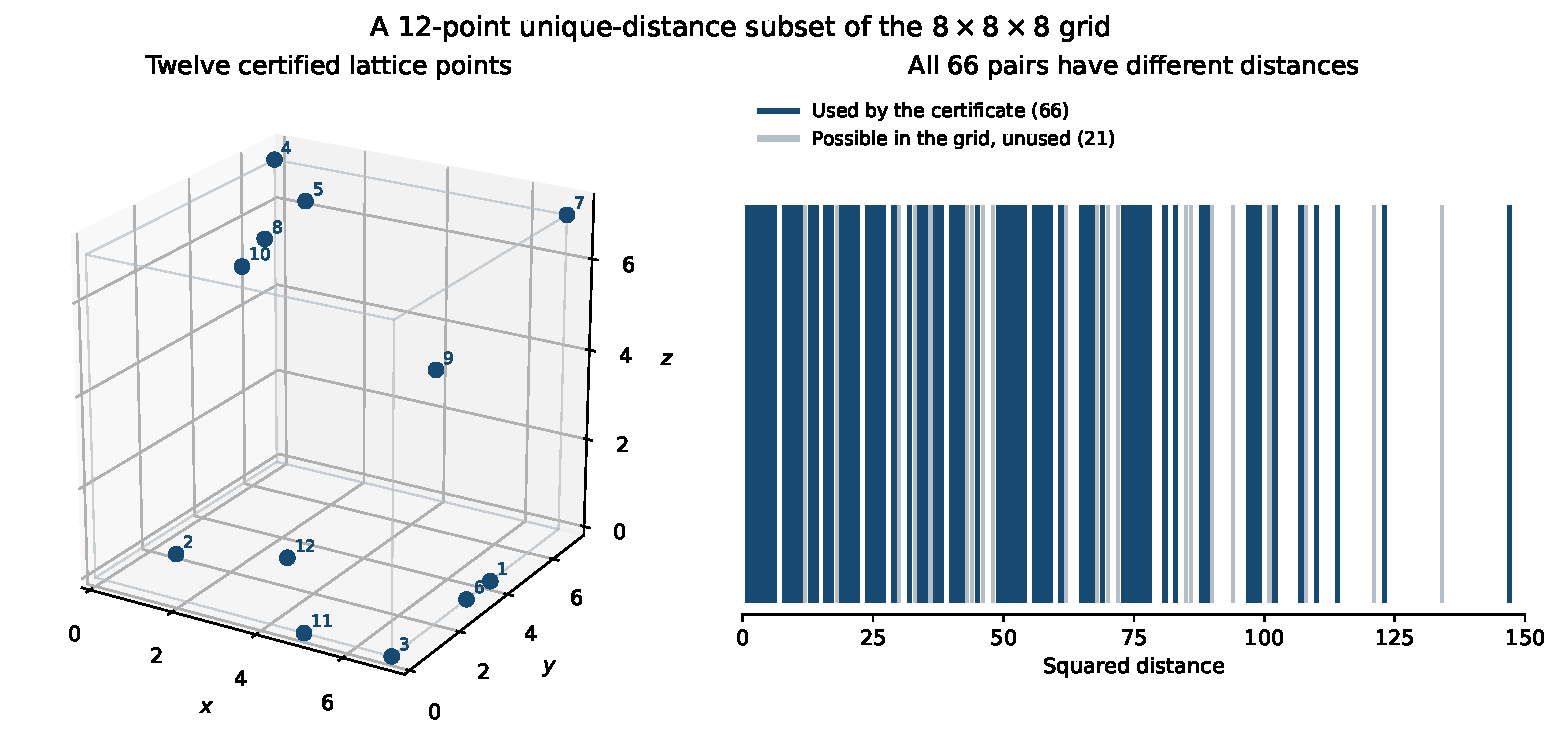
\includegraphics[width=\textwidth]{figures/witness_n8.pdf}
\caption{The 12-point witness in \(G_8\), with its exact squared-distance
spectrum. Gray marks are available cube distances that the witness does
not use. The 66 blue marks correspond to its 66 unordered pairs.}
\label{fig:witness}
\end{figure}
\[
\begin{aligned}
A_9=\{&(8,7,8),(4,0,2),(0,0,8),(2,0,8),\\
      &(8,8,0),(8,8,8),(4,8,0),(0,2,6),\\
      &(2,5,1),(3,4,2),(5,0,8),(3,3,1),(0,1,1)\}.
\end{aligned}
\]
The set \(A_9\) has 13 points and 78 distinct squared distances.
\[
\begin{aligned}
A_{10}=\{&(6,9,0),(9,3,6),(9,9,0),(0,0,1),\\
        &(1,0,9),(0,9,4),(9,8,1),(8,3,6),\\
        &(2,1,8),(7,7,0),(2,5,9),(6,0,9),\\
        &(9,8,3),(3,7,0)\}.
\end{aligned}
\]
The set \(A_{10}\) has 14 points and 91 distinct squared distances.

\subsection{A search that walks through valid configurations}
Collision-minimization searches found configurations with only one or
two repeated distances, but several stalled there. A more successful
procedure maintains a valid \(k\)-point set throughout. Delete three
points, or four with probability one third, leaving a fixed core. List
all grid points that are individually admissible against that core,
shuffle their order, and recursively refill while preserving distinctness.
A refill with one extra point proves a larger lower bound. An unsuccessful
bounded traversal can select a valid refill of the original size as the
next state.

This is a heuristic exploration of valid sets; a node cap limits each
move. The validity of every completed construction is exact, whereas
failure of a bounded traversal has no global meaning. With \(C\le n^3\)
remaining candidates and a traversal cap of \(B\) successful partial
refills, a safe per-move bound is \(O(n^3k+BCk)\). Counting only successful
partial refills does not count all failed candidate trials, so a claimed
\(O(Bk)\) bound would be unjustified.

The three displayed witnesses were found from valid starting sets in
497902, 109517, and 5858 moves respectively, with seeds 888112, 999123,
and 101314. Recorded wall times were approximately 108.75, 20.41,
and 1.29 seconds. These are warm-started search observations, not a
controlled comparison of algorithms or machines. The starting sets,
source code, and discovery metadata are included in the package.
A later version deletes four or five points per move. It produced
16 points in \(G_{12}\) and 18 points in \(G_{14}\), completing the
certified inequality \(a_n\ge n+4\) for every \(8\le n\le14\).
The immutable starting configurations and exact iteration budgets
for these runs are included as well.

\subsection{Certificate checks}
A separate Python verifier checks coordinate ranges, distinct points,
and a dictionary from squared distance to its unique unordered point
pair. It also verifies the full supplied distance inventory. Such a
check takes \(O(k^2)\) exact arithmetic operations for a witness of
size \(k\). No comparison of rounded Euclidean lengths is used.

\subsection{The complete finite catalogue through side length thirty}
All lower bounds in Table~\ref{tab:catalogue} have explicit coordinate
certificates. The upper bounds shown there are the elementary palette
and parity bounds; no exactness is asserted for these larger sizes.
\begin{table}[ht]
\centering
\caption{Certified bounds beyond side length ten. All point lists are supplied.}
\label{tab:catalogue}
\begin{tabular}{rrr@{\qquad}rrr}
\toprule
\(n\)&Lower&Upper&\(n\)&Lower&Upper\\
\midrule
11&15&19&21&22&38\\
12&16&21&22&23&40\\
13&17&23&23&24&42\\
14&18&24&24&25&43\\
15&18&26&25&26&46\\
16&18&28&26&26&48\\
17&19&30&27&27&50\\
18&20&32&28&28&52\\
19&21&34&29&29&54\\
20&22&36&30&30&55\\
\bottomrule
\end{tabular}
\end{table}



\section{Arithmetic density without a three-square sufficiency theorem}
\label{sec:arithmetic}
For the upper bounds it is enough to use the arithmetic superset
\[
 \calB=\NN_{>0}\setminus
 \{4^a(8b+7):a,b\in\NN\}.
\]
Every positive sum of three integer squares belongs to \(\calB\).
To see this, note that a square modulo 8 is 0, 1, or 4, and three such
squares cannot sum to 7 modulo 8. If a sum of three squares is divisible
by 4, reducing modulo 4 shows that all three coordinates are even.
Divide by 4 and repeat. The converse assertion, namely that every
member of \(\calB\) is a sum of three squares, is not needed here.

\begin{lemma}[Admissible-integer counting]
\label{lem:count}
Let \(B(X)=|\calB\cap[1,X]|\). Then
\begin{equation}
 B(X)=\frac56X+O(\log(2+X)).
 \label{eq:density}
\end{equation}
For every fixed continuously differentiable \(f:[0,3]\to\RR\),
\begin{equation}
 \sum_{\substack{r\in\calB\\r\le3N^2}}f(r/N^2)
 =\frac56N^2\int_0^3f(t)\,dt+O_f(\log(2+N)).
 \label{eq:weighted-density}
\end{equation}
\end{lemma}
\begin{proof}
The excluded progressions \(4^a(8b+7)\) are disjoint, since the exact
power of 4 dividing such a number identifies \(a\). For \(X\ge1\),
\[
 B(X)=\floor X-
 \sum_{a\ge0}
 \floor{\frac{\floor{X/4^a}+1}{8}}.
\]
There are \(O(\log(2+X))\) nonzero terms. Each is
\(X/(8\cdot4^a)+O(1)\), and the omitted tail of the main geometric
series is \(O(1)\). Since
\(\sum_{a\ge0}(8\cdot4^a)^{-1}=1/6\), this proves
\cref{eq:density}. Partial summation, with the derivative of
\(f(t/N^2)\) contributing a factor \(N^{-2}\), gives
\cref{eq:weighted-density}.
\end{proof}

The elementary arithmetic upper bound is consequently
\[
 \binom{a_n}{2}\le B(3(n-1)^2)
 =\frac52(n-1)^2+O(\log n),
 \qquad a_n\le\sqrt5(n-1)+O(1).
\]
This bounds the exact cube palette by an arithmetic superset. It does
not assert an asymptotic equality for \(d_n\).

\subsection{A limitation of the modulo-four counting relaxation}
The leading counts of members of \(\calB\cap[1,3N^2]\) in residues
\(0,1,2,3\pmod4\) are
\[
 \left(\frac58,\frac34,\frac34,\frac38\right)N^2.
\]
For residue zero this follows by dividing by four and applying
\cref{lem:count}; residues one and two have density \(1/4\) each,
and the allowed odd residue-three integers are precisely \(3\pmod8\).

These four arithmetic capacities alone cannot improve the leading
coefficient \(\sqrt5\). To see this, put
\[
 u=\frac1{\sqrt{10}},\qquad v=\frac1{\sqrt5},\qquad
 p_{000}=\frac{1+4u+3v}{8},\quad
 p_{111}=\frac{1-4u+3v}{8},
\]
and give each of the other six classes mass \((1-v)/8\).
These are positive masses summing to one. For two independent
parity classes with this distribution, direct substitution gives
Hamming-distance probabilities
\[
 (P_0,P_1,P_2,P_3)=
 \left(\frac14,\frac3{10},\frac3{10},\frac3{20}\right).
\]
At \(m\sim\sqrt5N\), the leading requirements
\(\tfrac12m^2P_r\) equal the four capacities above. For any fixed
\(0<c<\sqrt5\), choose integer occupancies of total size
\(m=\floor{cN}\) approximating these proportions. Rounding changes
each requirement by \(O(N)\), while the capacity slack is
\(\Theta(N^2)\), so every constraint is eventually satisfied.
This constructs feasible arithmetic occupancies. Geometric
realizability, and the effect of the exact bounded-coordinate palette,
require additional information.

\section{Positive-definite kernels turn geometry into a stronger bound}
\label{sec:kernel}
Fix \(\lambda>0\). For probability measures \(\mu,\eta\) on the unit
cube, define
\[
 K_\lambda(x,y)=e^{-\lambda\norm{x-y}^2},\qquad
 \calE_\lambda(\mu,\eta)=
 \iint K_\lambda(x,y)\,d\mu(x)\,d\eta(y),
 \qquad \calE_\lambda(\mu)=\calE_\lambda(\mu,\mu).
\]

\begin{lemma}[Gaussian positivity]
\label{lem:pd}
Every finite signed measure \(\sigma\) on \([0,1]^3\) satisfies
\(\calE_\lambda(\sigma)\ge0\).
\end{lemma}
\begin{proof}
Use the uniformly convergent expansion on the compact product cube
\[
 K_\lambda(x,y)
 =e^{-\lambda\norm{x}^2}e^{-\lambda\norm{y}^2}
 \sum_{\beta\in\NN^3}\frac{(2\lambda)^{|\beta|}}{\beta!}x^\beta y^\beta.
\]
Integrating term by term gives
\[
 \calE_\lambda(\sigma)=
 \sum_{\beta\in\NN^3}\frac{(2\lambda)^{|\beta|}}{\beta!}
 \left(\int e^{-\lambda\norm{x}^2}x^\beta\,d\sigma(x)\right)^2
 \ge0.
\]
\end{proof}

\begin{theorem}[Product-potential certificate]
\label{thm:kernel}
Let \(\nu\) be a probability measure on \([0,1]\), with potential and
energy
\[
 U_\nu(t)=\int e^{-\lambda(t-s)^2}\,d\nu(s),\qquad
 E_\nu=\int U_\nu(t)\,d\nu(t).
\]
Suppose
\[
 U_\nu(t)\ge u>0\quad(0\le t\le1),\qquad E_\nu\le e,
 \qquad \kappa=2u^3-e^3>0.
\]
Then every distance-distinct set of \(m\) points in \(G_n\), \(n\ge2\),
with \(N=n-1\), satisfies
\begin{equation}
 \kappa m^2\le m+2\sum_{r\in\calD_n}e^{-\lambda r/N^2}.
 \label{eq:finite-kernel-exact}
\end{equation}
In particular,
\begin{equation}
 \limsup_{n\to\infty}\frac{a_n}{n}
 \le
 \left(\frac{5(1-e^{-3\lambda})}{3\lambda\kappa}\right)^{1/2}
 \le\left(\frac5{3\lambda\kappa}\right)^{1/2}.
 \label{eq:kernel-asymptotic}
\end{equation}
\end{theorem}
\begin{proof}
Let \(\eta=\nu^{\otimes3}\). Its potential factors into three
one-dimensional potentials, so it is at least \(u^3\) throughout the
cube, and \(\calE_\lambda(\eta)=E_\nu^3\le e^3\).
Apply \cref{lem:pd} to \(\mu-\eta\):
\[
 \calE_\lambda(\mu)
 \ge2\calE_\lambda(\mu,\eta)-\calE_\lambda(\eta)
 \ge2u^3-e^3=\kappa.
\]
Now take \(\mu\) to be the empirical probability measure on the
selected points after division by \(N\). The diagonal terms each equal
1, and the off-diagonal terms occur twice, giving
\[
 \kappa m^2
 \le m+2\sum_{\{x,y\}\subset A}e^{-\lambda\norm{x-y}^2/N^2}.
\]
All squared distances are distinct members of \(\calD_n\), which proves
\cref{eq:finite-kernel-exact}. Enlarge the palette to
\(\calB\cap[1,3N^2]\), apply \cref{lem:count} with
\(f(t)=e^{-\lambda t}\), and obtain
\[
 \kappa m^2\le m+
 \frac53N^2\frac{1-e^{-3\lambda}}{\lambda}+O(\log N).
\]
The already proved estimate \(m=O(N)\) allows division by \(N^2\) and
passage to the limsup. Finally \(N/n\to1\).
\end{proof}

The method has two independently checkable inputs. Arithmetic bounds
how much total kernel weight distinct squared distances can consume.
A probability measure certifies a geometric lower bound on the kernel
energy of \emph{every} point distribution in the cube. This is why the
argument contains more information than counting available colors.

\begin{proposition}[Tensorization of the Gaussian energy minimum]
\label{prop:tensorization}
Let \(e_1(\lambda)\) be the minimum Gaussian energy over probability
measures on \([0,1]\). The minimum energy over probability measures
on \([0,1]^3\) is exactly \(e_1(\lambda)^3\).
\end{proposition}
\begin{proof}
Continuity of the kernel and compactness give a one-dimensional
minimizer \(\nu_*\). Varying it toward a point mass at \(x\), the
right derivative of the energy at zero is
\(2(U_{\nu_*}(x)-e_1(\lambda))\), which must be nonnegative.
Thus \(U_{\nu_*}\ge e_1(\lambda)\) everywhere. The product measure
\(\nu_*^{\otimes3}\) has energy \(e_1(\lambda)^3\), and the proof of
\cref{thm:kernel} with \(u=e=e_1(\lambda)\) shows that no cube
probability measure has smaller energy.
\end{proof}

This identifies a limitation and an advantage of the method. For a
fixed Gaussian kernel, optimizing a one-dimensional measure is enough
to obtain the best possible universal energy lower bound. A
nonproduct reference measure cannot improve that optimum. Stronger
information must come from a different kernel, additional arithmetic
or geometric constraints, or a sharper use of the distance palette.

\section{A completely analytic certificate}
\label{sec:analytic-certificate}
Set
\[
 \lambda=4\log6,\quad \alpha=\log6,\quad
 \nu=\frac{216}{605}(\delta_0+\delta_1)
       +\frac{173}{605}\delta_{1/2},\quad
 E=\frac{49}{121}.
\]
The masses are nonnegative and sum to one.

\begin{lemma}
\label{lem:analytic-potential}
For this measure, \(U_\nu(x)\ge E\) on \([0,1]\), with equality at
\(0,1/2,1\). Consequently \(E_\nu=E\).
\end{lemma}
\begin{proof}
Put \(t=2x-1\). Direct substitution gives
\[
 605U_\nu(x)=e^{-\alpha t^2}
 \bigl[72\cosh(2\alpha t)+173\bigr].
\]
The required inequality is
\[
 F(t):=72\cosh(2\alpha t)+173-245e^{\alpha t^2}\ge0
 \quad(|t|\le1).
\]
There is equality at \(t=0\). At \(t=1\),
\[
 72\frac{6^2+6^{-2}}2+173=245\cdot6,
\]
so \(F(1)=0\) as well.

For \(k\ge1\), the ratio between the positive cosh contribution and
the exponential contribution to the coefficient of \(t^{2k}\) is
\[
 r_k=\frac{72}{245}\frac{(2\alpha)^k}{(2k-1)!!},
 \qquad \frac{r_{k+1}}{r_k}=\frac{2\alpha}{2k+1}.
\]
The rational bounds \(1.79<\alpha<1.80\) imply
\[
 r_1=\frac{144\alpha}{245}>1,\qquad
 r_2=\frac{96\alpha^2}{245}>1,\qquad
 r_3=\frac{192\alpha^3}{1225}<1.
\]
For \(k\ge3\) the ratios continue decreasing. Therefore
\[
 F(t)=b_1t^2+b_2t^4-\sum_{k\ge3}c_kt^{2k},
 \qquad b_1,b_2,c_k>0.
\]
Absolute convergence and \(|t|\le1\) give
\[
 F(t)\ge t^4\left(b_1+b_2-\sum_{k\ge3}c_k\right)
 =t^4F(1)=0.
\]
The support equalities prove \(E_\nu=E\).
\end{proof}

For completeness, the two coarse logarithm bounds used in the proof
can be checked by rational arithmetic from
\[
 \log6=2\sum_{j\ge0}\frac{(5/7)^{2j+1}}{2j+1}.
\]
After the first \(J\) terms, the tail is at most
\[
 \frac{2(5/7)^{2J+1}}{(2J+1)(1-(5/7)^2)}.
\]
Taking \(J=10\) proves \(179/100<\log6<9/5\).

\begin{corollary}
The analytic bound \cref{eq:main-analytic} holds.
\end{corollary}
\begin{proof}
Use \(u=e=E\), so \(\kappa=E^3\), in \cref{thm:kernel}.
Since \(e^{-3\lambda}=6^{-12}\), its coefficient is exactly \(C_6\).
\end{proof}

The proof also identifies an actual Gaussian-energy minimizer on the
cube, namely \(\nu^{\otimes3}\), for this value of \(\lambda\):
its energy is \(E^3\), and no probability measure has smaller energy.
This statement concerns a continuous energy problem; it does not
construct a large lattice configuration with distinct distances.

\section{The stronger four-atom certificate}
\label{sec:computer-certificate}
The stronger certificate uses \(\lambda=10\) and the rational measure
\[
 \nu=
 \frac{3183}{10000}(\delta_0+\delta_1)
 +\frac{1817}{10000}
  (\delta_{3791/10000}+\delta_{6209/10000}).
\]
All parameters in the verifier are exact integers. Set
\begin{equation}
 u=\frac{36532567}{10^8},\qquad
 e=\frac{36533029}{10^8}.
 \label{eq:ue}
\end{equation}

\begin{proposition}[Verified potential inequalities]
\label{prop:verified-potential}
The accompanying integer-arithmetic verification proves
\[
 U_\nu(x)\ge u\quad(0\le x\le1),\qquad E_\nu\le e.
\]
\end{proposition}
\begin{proof}
The finite checks and the passage from a mesh to the entire interval
are as follows.

\paragraph{Exponential intervals.}
All mesh and support differences are \(d/10000\), \(0\le d\le10000\).
To bound \(e^{-10(d/10000)^2}\), divide the exponent by 16:
\[
 y=\frac{d^2}{160000000}\in[0,5/8].
\]
The alternating Taylor sums satisfy
\[
 S_{21}(y)\le e^{-y}\le S_{20}(y),\qquad
 S_j(y)=\sum_{k=0}^j\frac{(-y)^k}{k!}.
\]
The terms decrease in magnitude on this interval. Each sum is evaluated
outward on a fixed-point scale \(10^{40}\), and four outward-rounded
squarings enclose the original exponential. Every operation is an
integer multiplication, division, or comparison.

\paragraph{Potential on a mesh.}
Evaluate the four-term potential at \(x=i/10000\).
Reflection symmetry reduces the computation to \(0\le i\le5000\).
The smallest certified lower value occurs at \(i=3792\) and is greater
than
\[
 0.36532569867781706035.
\]
This displayed decimal is only a readable summary of a rational bound;
the verifier does not use decimal rounding to justify an assertion.

\paragraph{Interpolation between mesh points.}
For \(g(x)=e^{-\lambda(x-y)^2}\),
\[
 |g''(x)|=
 2\lambda\,|2z-1|e^{-z}\le2\lambda,\qquad
 z=\lambda(x-y)^2\ge0.
\]
Indeed, the maximum of \(|2z-1|e^{-z}\) is 1. Since the weights sum
to one, \(|U_\nu''|\le20\). A twice differentiable function differs
from its linear interpolant on an interval of length \(h\) by at most
\(20h^2/8\). Here this is \(1/40000000\).
Subtracting that quantity from the mesh lower bound gives more than
\[
 0.36532567367781706035>u.
\]
Thus the check covers every real \(x\), not just the sampled mesh.

\paragraph{Energy.}
The 16 weighted support-to-support kernel terms, evaluated with upper
exponential intervals, give
\[
 E_\nu<0.36533028829202422565<e.
\]
The script checks both final rational inequalities exactly.
\end{proof}

\begin{theorem}[Certified asymptotic coefficient]
\label{thm:certified}
Let
\[
 \kappa=2u^3-e^3
 =\frac{48755553510102913673137}{10^{24}}>0.
\]
Then
\[
 \limsup_{n\to\infty}\frac{a_n}{n}
 \le\sqrt{\frac1{6\kappa}}
 =1.848895345708975128\ldots<1.849.
\]
\end{theorem}
\begin{proof}
Apply \cref{thm:kernel} with \(\lambda=10\) and
\cref{prop:verified-potential}. Dropping the positive factor
\(e^{-30}\) from \(1-e^{-30}\) only enlarges the upper bound:
\(5/(3\lambda)=1/6\). The inequality
\[
 \frac1{6\kappa}<\left(\frac{1849}{1000}\right)^2
\]
is an exact rational comparison performed by the verifier.
\end{proof}

The certificate file contains the chosen rational bounds, the exact
\(\kappa\), the interval parameters, and the resulting constant.
The verifier is short enough to audit independently and needs only
Python's standard library. Floating-point square roots are unnecessary
for verification; decimal values are printed only after the rational
inequalities have passed.

\begin{figure}[ht]
\centering
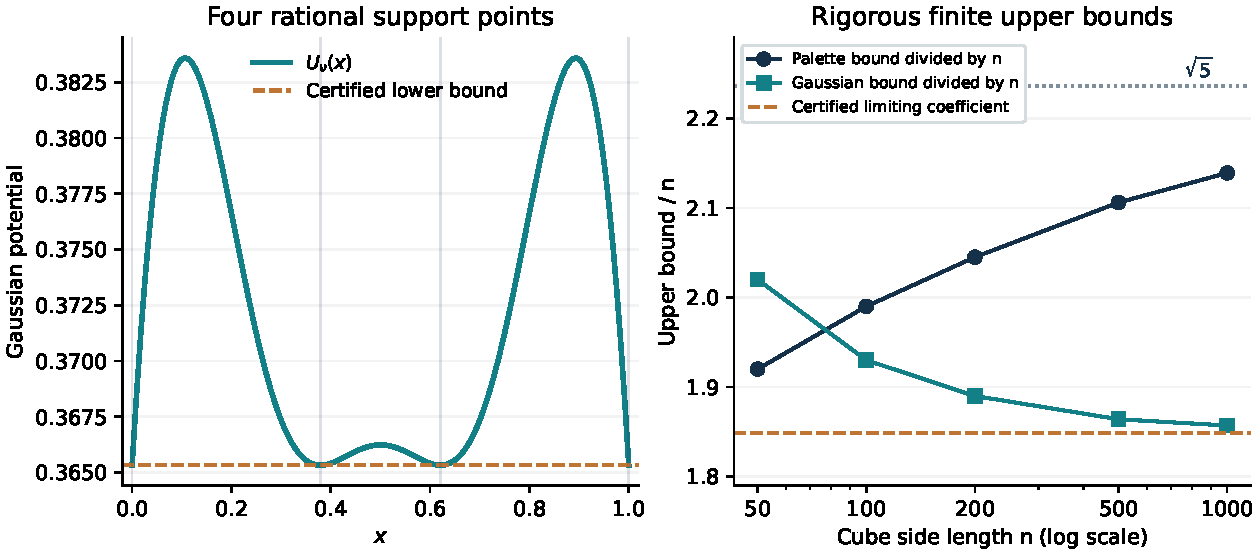
\includegraphics[width=\textwidth]{figures/kernel_bounds.pdf}
\caption{Left: the four-atom potential, illustrated numerically; the
proof of its global lower bound is the exact interval certificate.
Right: computed finite upper bounds divided by the side length.
These curves bound \(a_n/n\); they are not measured values of that ratio.
The dotted line is the elementary coefficient \(\sqrt5\).}
\label{fig:kernel}
\end{figure}

\section{Rigorous finite upper bounds from the same certificate}
\label{sec:finite-kernel}
For \(N=n-1\) and \(\delta=10/N^2\), the infinite admissible-distance
Laplace sum has the exact identity
\begin{equation}
 W_\infty(\delta)=
 \sum_{r\in\calB}e^{-\delta r}
 =\frac{e^{-\delta}}{1-e^{-\delta}}
 -\sum_{a\ge0}
 \frac{e^{-7\delta4^a}}{1-e^{-8\delta4^a}}.
 \label{eq:geometric}
\end{equation}
This follows by subtracting the disjoint forbidden progressions.
For any nonnegative integer \(A\), truncating the subtraction after
\(a=A-1\) gives an \emph{upper} bound \(W_A\) for \(W_\infty\).
Enlarging \(\calD_n\) to all of \(\calB\) is also an upper bound.
Consequently
\begin{equation}
 \kappa a_n^2-a_n\le2W_A,\qquad
 a_n\le
 \floor{\frac{1+\sqrt{1+8\kappa W_A}}{2\kappa}}.
 \label{eq:finite-rational}
\end{equation}

The supplied \code{finite\_bounds.py} evaluates an upper enclosure of
\(W_A\) entirely with rational arithmetic. It bounds the first geometric
series from above and each subtracted series from below. Terms whose
initial exponent exceeds 56 are left unsubtracted. Exponentials are
reduced by a factor of 128, enclosed with alternating Taylor sums of
degrees 31 and 30, and raised by seven directed squarings. The largest
integer satisfying the resulting quadratic inequality is located by
integer comparisons; numerical root rounding cannot affect the answer.

\begin{table}[ht]
\centering
\caption{Upper bounds computed with exact arithmetic. The Gaussian column
uses \cref{eq:finite-rational}, not an asymptotic expression rounded at
finite \(n\).}
\label{tab:large-upper}
\begin{tabular}{rrrrr}
\toprule
\(n\)&\(d_n\)&Palette&Parity&Gaussian\\
\midrule
50&4606&96&96&101\\
100&19798&199&199&193\\
200&83752&409&409&378\\
500&554119&1053&1052&932\\
1000&2287097&2139&2138&1857\\
\bottomrule
\end{tabular}
\end{table}

The diagonal term \(a_n\) in the energy inequality makes this version
weak for very small cubes. One should take the minimum of the available
bounds. At larger side lengths the Gaussian bound improves the
arithmetic palette bound by a substantial margin. For example,
\[
 a_{100}\le193,\qquad a_{500}\le932,\qquad a_{1000}\le1857.
\]
These are upper bounds, not computed sequence terms.
The counting estimate also gives the more precise upper-bound
expansion
\[
 a_n\le C_{\rm cert}(n-1)+\frac1{2\kappa}
       +O\!\left(\frac{\log n}{n}\right).
\]
It follows by inserting
\(2W_\infty(10/(n-1)^2)=(n-1)^2/6+O(\log n)\) into the quadratic
inequality. This is an expansion of an upper bound, not an asymptotic
formula for \(a_n\), and its unspecified remainder should not be
rounded to obtain finite certified integers.

\section{Lower bounds and why the exponent two thirds appears}
\label{sec:lower}

\subsection{An exact finite alteration inequality}
For each squared distance \(d\), let \(H_d\) be its graph on \(G_n\),
with \(e_d\) edges and vertex degrees \(\deg_d(v)\). Define
\[
 T=\sum_d\sum_{v\in G_n}\binom{\deg_d(v)}2,\qquad
 Q=\sum_d\binom{e_d}2-T.
\]
Here \(T\) counts pairs of equal-length edges sharing a vertex, and
\(Q\) counts such pairs with disjoint endpoints.

\begin{proposition}[Sampling and deletion]
\label{prop:alteration}
For every \(0\le p\le1\),
\[
 a_n\ge
 \ceil{p n^3-p^3T-p^4Q}.
\]
\end{proposition}
\begin{proof}
Retain every grid point independently with probability \(p\).
The expected number retained is \(pn^3\). A conflict with three
distinct endpoints survives with probability \(p^3\), and one with
four survives with probability \(p^4\). Delete one point from each
surviving conflict, if that conflict has not already been destroyed.
Deletion cannot create a new equality between distances.
The final valid set has size at least the number retained minus the
number of surviving conflicts. Some outcome is at least its expected
lower bound, and the size is integral.
\end{proof}

This is a constructive randomized procedure, although listing all
conflicts can be expensive. It is also a useful accounting device:
overcounting conflicts weakens the lower bound but does not invalidate it.

\subsection{An elementary equal-norm energy estimate}
\begin{lemma}
\label{lem:equal-norm}
The number of ordered pairs \(u,v\in[-N,N]^3\cap\mathbb Z^3\) with
\(\norm{u}^2=\norm{v}^2\) is \(O(N^4)\).
\end{lemma}
\begin{proof}
Put \(a=u-v\), \(b=u+v\). This is an injective map into pairs
\(a,b\in[-2N,2N]^3\) with \(a\cdot b=0\). Ignoring the parity
condition needed to recover \(u,v\) only enlarges the count.
The case \(a=0\) contributes \(O(N^3)\).

For \(a\ne0\), write \(a=g a_0\), where \(a_0\) is primitive,
\(r=\norm{a_0}_\infty\), and \(1\le g\le2N/r\).
Permute coordinates so that \(|(a_0)_3|=r\), and put
\(h=\gcd((a_0)_2,r)\). Primitivity implies
\(\gcd((a_0)_1,h)=1\). The congruence
\[
 (a_0)_1b_1+(a_0)_2b_2\equiv0\pmod r
\]
forces \(h\mid b_1\). There are at most \(4N/h+1\) possibilities
for \(b_1\). For each, \(b_2\) occupies one residue class modulo
\(r/h\), giving at most \(4Nh/r+1\) possibilities. The equation
then determines \(b_3\) uniquely, if it is in range. Thus the number
of \(b\)'s is at most
\[
 \left(\frac{4N}{h}+1\right)
 \left(\frac{4Nh}{r}+1\right)
 \le\frac{16N^2}{r}+8N+1.
\]
There are at most
\((2r+1)^3-(2r-1)^3=24r^2+2\) choices for a primitive \(a_0\)
of sup norm \(r\). Summing the upper bound
\[
 \sum_{r=1}^{2N}
 (24r^2+2)\frac{2N}{r}
 \left(\frac{16N^2}{r}+8N+1\right)
\]
gives \(O(N^4)\). The terms involving \(1/r\) or \(1/r^2\) are
smaller than that order, so no extra logarithm is required.
\end{proof}

\begin{corollary}[Elementary polynomial lower bound]
\label{cor:elementary-lower}
There is an absolute \(c_0>0\) such that
\(a_n\ge c_0 n^{2/3}\) for all sufficiently large \(n\).
\end{corollary}
\begin{proof}
Let \(r_3(d)\) count displacement vectors of squared norm \(d\)
in \([-(n-1),n-1]^3\). The preceding lemma gives
\(\sum_d r_3(d)^2=O(n^4)\). Since
\(\deg_d(v)\le r_3(d)\) and \(e_d\le n^3r_3(d)/2\),
\[
 T=O(n^7),\qquad Q=O(n^{10}).
\]
Choose \(p=\gamma n^{-7/3}\), where \(\gamma>0\) is a sufficiently
small constant. The alteration bound becomes
\[
 pn^3-p^3T-p^4Q
 \ge\bigl(\gamma-C\gamma^4\bigr)n^{2/3}-C'\gamma^3.
\]
For a suitable fixed \(\gamma\), the leading coefficient is positive.
\end{proof}

The exponent arises from balancing retained vertices against
four-vertex conflicts: \(pn^3\) and \(p^4n^{10}\) have the same
order when \(p\asymp n^{-7/3}\). The three-vertex conflicts are of
lower order at that scale.

The logarithmic improvement in \cref{eq:LT} comes from the stronger
hypergraph analysis of Lefmann and Thiele \cite{lt,ltreport}. The
elementary proof above explains the scale, but it is not an improvement
over their theorem. In particular, the newly generated finite
configurations do not establish a linear lower bound.

\section{Structural properties and monotonicity}
\label{sec:structure}

\subsection{Properties that follow immediately}
The sequence is nondecreasing, because \(G_n\subseteq G_{n+1}\).
It is unbounded by \cref{eq:LT}, or by embedding successively longer
finite Golomb rulers on a coordinate line. Consequently there are
infinitely many strict increases.

Translations, cube isometries, and nonzero uniform integer dilations
preserve distinctness. Restricting a valid configuration to a subbox
also preserves it. More generally, for the rectangular-box extremal
function \(F(l_1,l_2,l_3)\), cutting one coordinate interval gives
\[
 F(l_1+l'_1,l_2,l_3)
 \le F(l_1,l_2,l_3)+F(l'_1,l_2,l_3).
\]
No requirement is imposed on distances crossing the cut when deriving
this upper bound, so the inequality is valid.

All nonzero ordered difference vectors of a valid configuration are
distinct. In the usual additive terminology it is therefore a Sidon
configuration. The converse fails: different displacement vectors,
such as \((1,0,0)\) and \((0,1,0)\), can have the same norm.
Likewise, a Cartesian product usually fails because translated copies
repeat every internal distance. These observations explain why
standard additive constructions require additional work here.

\subsection{Limiting measures of linearly sized configurations}
Compactness supplies weakly convergent subsequences of the scaled
empirical measures. The next result therefore applies to every
positive subsequential ratio of configuration size to side length.
\begin{proposition}[A bounded squared-distance density]
\label{prop:limiting-law}
Suppose \(n_j\to\infty\), \(N_j=n_j-1\), and valid configurations
\(A_j\subseteq G_{n_j}\) have sizes \(m_j\) with
\(m_j/N_j\to c>0\). Let their empirical probability measures after
scaling by \(N_j^{-1}\) converge weakly to \(\mu\) on the unit cube.
If \(\rho_\mu\) is the law of \(\norm{X-Y}^2\) for independent
\(X,Y\) with law \(\mu\), then
\[
 \rho_\mu\le\frac5{3c^2}\,dt\quad\hbox{on }[0,3].
\]
In particular, this squared-distance law has a bounded density and
\(\mu\) has no atoms.
\end{proposition}
\begin{proof}
Write \(\mu_j\) and \(\rho_j\) for the finite empirical measures
and their squared-distance laws. Weak convergence on the compact
cube passes to product measures and then through the continuous
squared-distance map. For nonnegative \(f\in C^1[0,3]\), uniqueness
of the used distances gives
\[
 \int f\,d\rho_j
 =\frac{f(0)}{m_j}
 +\frac2{m_j^2}\sum_{d\,\mathrm{used}}f(d/N_j^2)
 \le\frac{f(0)}{m_j}
 +\frac2{m_j^2}\sum_{\substack{r\in\calB\\r\le3N_j^2}}f(r/N_j^2).
\]
Apply \cref{lem:count} and take the limit. The resulting inequality
\(\int f\,d\rho_\mu\le(5/(3c^2))\int_0^3f(t)\,dt\)
extends by approximation to every nonnegative continuous function,
which proves domination of measures. An atom of \(\mu\) would give
an atom of \(\rho_\mu\) at zero, so none is possible.
\end{proof}

For example, the proposition implies the uniform local bound
\[
 \mu(B(x,r))\le\sqrt{\frac{20}{3c^2}}\,r,
\]
because two points in that ball are at squared distance at most
\(4r^2\). A stronger dimensional statement follows from
\[
 I_s(\mu):=\iint\norm{x-y}^{-s}\,d\mu(x)d\mu(y)
 \le\frac5{3c^2}\,
 \frac{3^{1-s/2}}{1-s/2}<\infty\qquad(0<s<2).
\]
Every Borel set of positive \(\mu\)-measure therefore has Hausdorff
dimension at least two. Here is the relevant energy argument.
The potential \(\int\norm{x-y}^{-s}\,d\mu(y)\) is finite at
\(\mu\)-almost every \(x\). Inside any set of positive measure,
restrict to a positive-measure subset where that potential is at
most some finite \(M\). A ball of radius \(r\) centered in this
subset has \(\mu\)-mass at most \(Mr^s\). A covering by balls,
enlarged by a factor two to center them in the subset, then has
\(\sum r_i^s\) bounded away from zero. Its Hausdorff dimension
is at least \(s\); let \(s\) increase to two.

There is a useful continuous optimization problem behind this
constraint. Define
\[
 F(\mu)=\inf\{M\ge0:\rho_\mu\le M\,dt\},\qquad
 \beta=\inf_{\mu\in\mathcal P([0,1]^3)}F(\mu),
\]
allowing \(F(\mu)=\infty\). Since every squared-distance law has
mass one on an interval of length three, \(\beta\ge1/3\).
Every positive limiting ratio satisfies
\[
 c\le\sqrt{\frac5{3\beta}}.
\]
For any nonzero nonnegative continuous test function \(f\),
\[
 \beta\ge
 \frac{\displaystyle\inf_\mu
   \iint f(\norm{x-y}^2)\,d\mu(x)d\mu(y)}
      {\displaystyle\int_0^3f(t)\,dt}.
\]
The Gaussian argument is one instance of this inequality. Optimizing
over several tests or imposing the full density constraint offers
a systematic further relaxation. No interchange of infimum and
supremum, or strong-duality assertion, is needed here. Discrete
configurations approaching a feasible limiting measure would still
require a separate construction.

\subsection{Strict monotonicity would already be a strong theorem}
\begin{proposition}
\label{prop:strict}
If \(a_{n+1}>a_n\) for every sufficiently large \(n\), then
\[
 a_n\ge n-O(1).
\]
Thus eventual strict monotonicity would imply a linear lower bound.
If instead \(a_n=o(n)\), then among the first \(N\) transitions,
all but \(o(N)\) are plateaus.
\end{proposition}
\begin{proof}
The sequence is integral. Each strict increase is at least one, so
eventual strict increase telescopes to \(a_n\ge n-O(1)\).
Conversely, the number of strict increases up to \(N\) is at most
\(a_N-a_0\); under a sublinear upper bound this is \(o(N)\).
\end{proof}

The known asymptotic bounds do not decide between these alternatives.
The small computed terms increase, but that observation does not
establish strict increase indefinitely. A proof of strict monotonicity
would do much more than settle a local-looking sequence question: it
would close the known exponent gap in favor of order \(n\).

\subsection{What the evidence does and does not suggest}
The now-known exact values satisfy
\[
 a_n=\floor{3n/2}\qquad(0\le n\le8).
\]
This is a finite observation and a reasonable target for the next
searches. No argument here supports extrapolating the formula to all
\(n\). Such a formula would, in particular, supply a linear lower
bound and resolve the exponent question, far beyond the currently
established construction theorem.

The small values and the available constructions are useful search
targets. They are not enough to select a growth exponent by regression.
The interval between the known lower and upper bounds is still wide;
finite-size effects and heuristic search quality both affect the
observed ratios.

The proper current conclusion from this report is
\[
 c\,n^{2/3}(\log n)^{1/3}
 \le a_n
 \le (1.848895345709\ldots+o(1))n.
\]
There is no general formula proved here, no proof of \(\Theta(n)\),
and no proof of \(o(n)\).

\section{Further research questions and a concrete next program}
\label{sec:future}

\begin{enumerate}[label=\textbf{\arabic*.},leftmargin=*]
\item \textbf{Continue exact terms with independently checked
impossibility proofs.}
The next unproved target sizes in the finite table should be searched
using the unique-diameter split. Preserve a record for every case and
avoid collapsing partial UNSAT results into a global conclusion.
Translate promising instances into SAT or pseudo-Boolean form and
request a proof trace that a separate checker can verify.

\item \textbf{Optimize complete geometric case splits.}
Diameter anchoring is effective because the high-distance palette
forces endpoints toward the boundary. The computations already
demonstrate the benefit of anchoring several largest edges. The next
questions are how to select the prefix length adaptively and how to
use its incidence pattern before enumerating endpoints. The covering
argument must explicitly allow these edges to share endpoints.

\item \textbf{Use arithmetic occupancy beyond modulus four.}
Modulo-four coordinate parity has only eight classes and is cheap.
Moduli eight, three, or five retain more information but create larger
occupancy spaces. A useful goal is a hierarchy that tightens bounds
without spending more time on the relaxation than it saves in search.
An infeasible modular relaxation should produce a compact arithmetic
certificate.

\item \textbf{Improve lower-bound search and publish reusable witnesses.}
Tabu search, deletion and exact refill, and adaptive vertex moves can
be combined with an archive of high-quality configurations. Preserve
the full point lists, deterministic iteration budgets, and checksums.
Transfer a solution from \(G_n\) into \(G_{n+1}\), then search for an
extension or a small replacement. Failure of that local neighborhood
must remain a local statement.

\item \textbf{Optimize the kernel certificate.}
Vary \(\lambda\), the support positions, and the masses in one
dimension; then verify every resulting improvement by interval
arithmetic or analytic inequalities. Mixtures of Gaussians are
positive definite and may better exploit the shape of the admissible
distance set. By \cref{prop:tensorization}, nonproduct reference
measures cannot improve the optimum for a single Gaussian. Mixtures
no longer have the same product factorization and lead to a different
continuous energy problem, where correlations may matter.

\item \textbf{Combine kernels with congruence information.}
The Gaussian bound uses only the density \(5/6\) of an arithmetic
superset of distances. Periodic weights or residue-indexed positive
semidefinite kernels could incorporate parity capacities directly
into the continuous energy problem. Positivity must be proved for
the combined kernel, not inferred from a numerical matrix sample.
The full bounded-density relaxation in \cref{prop:limiting-law}
provides another systematic target. Determine or bound \(\beta\),
and study whether its minimizing measures can arise as limits of
discrete configurations.

\item \textbf{Resolve the growth exponent.}
Does \(a_n=n^{2/3+o(1)}\), does \(a_n=n^{1-o(1)}\), or is the exponent
intermediate? An upper bound \(O(n^{1-\varepsilon})\), or a lower
bound \(n^{2/3+\varepsilon}\), would represent a substantially larger
advance than improving the linear coefficient.

\item \textbf{Understand the exact box palette asymptotically.}
Determine the deficit between \(|\calD_n|\) and
\(B(3(n-1)^2)\). The coordinate cap excludes representations near
the boundary, and unrestricted three-square representability alone
does not quantify that deficit. A sharp error term would improve
finite bounds and clarify how much of the obstruction is arithmetic
versus geometric.

\item \textbf{Construct the known lower-bound scale explicitly.}
The hypergraph existence theorem has a strong asymptotic guarantee,
but a usable implementation with explicit constants would make it
possible to compare that guarantee with optimization heuristics.
Derandomization by conditional expectation is another concrete
direction.

\item \textbf{Settle strict monotonicity or find the first plateau.}
This question should be pursued together with the asymptotic problem,
in view of \cref{prop:strict}. A plateau needs an exact upper
certificate on the larger cube and a matching witness on the smaller
one. A general extension theorem would need to control all new
distances simultaneously.
\end{enumerate}

\appendix
\section{How to reproduce and inspect the package}
\label{app:reproduce}

The root of the ZIP contains this document's \code{a275672.tex} and
compiled PDF. The \code{src} directory contains independent
certificate verifiers and the exact finite-bound calculator.
The \code{data} directory contains coordinates and verified numerical
results. Search source snapshots and retained run records are in
\code{computations/exact}; constructive programs and immutable starting
configurations are in \code{computations/constructions}. The
\code{validation} directory contains the separate source audit and
small-instance comparisons against an exhaustive reference enumerator.
Its \code{fresh\_audit} subdirectory contains a second independent
source review, differential tests, and sanitizer-run records. The
\code{computations/exploratory} directory retains explicitly
inconclusive larger-case attempts and the later filtered sources.

The numerical bounds can be regenerated with Python 3:
\begin{lstlisting}
python3 src/verify_results.py
python3 src/verify_gaussian_certificate.py
python3 src/finite_bounds.py 50 100 200 500 1000
\end{lstlisting}
The first command checks the complete construction catalogue, the
diameter-case coverage of the exact runs, arithmetic lemmas, and an
independent rational implementation of the potential certificate. The
second runs the original rational potential verifier. The third uses
rational exponential intervals and prints rigorous finite upper
bounds. None requires a numerical optimization library.

The C++ search programs require a C++17 compiler. Full target searches
may run substantially longer than witness checks. The README gives the
exact invocation and source version for each completed case run. A
reported time limit, an interruption, or a partial-case run must never
be interpreted as a proof for the entire cube.
The validated front end \code{src/run\_exact.py} checks arguments and
builds the selected source automatically; for example,
\begin{lstlisting}
python3 src/run_exact.py 8 13 --mode top6 --seconds 3600
\end{lstlisting}
It also resolves trivially oversized targets before they reach the
unchanged historical C++ sources, whose signed-integer pair-count
expression assumes an ordinary target within the supported grid.

The PDF can be rebuilt with \code{latexmk -pdf a275672.tex}. Standard
LaTeX packages and the included figure assets suffice; no Internet
access is needed for the rebuild. The supplied checksum manifest records
the packaged artifacts used for the reported computations.


\section{An independent geometric bound}
\label{app:geometric}
This optional argument gives the weaker coefficient
\[
 C_{\rm geom}=\frac{15\sqrt3-\sqrt{15}}{11}
 =2.0097980697\ldots.
\]
It is included because it uses geometric concentration rather than
positive-definite kernels.

If \(r_1<\cdots<r_s\) are distinct members of \(\calB\),
\cref{lem:count} implies
\[
 \sum_{j=1}^s r_j
 \ge\frac35s^2-O(s\log(s+2)).
\]
Choose a subsequence with \(m/N\to c>0\); the case \(c=0\) is
immediate. For the corresponding empirical measures, normalized to the
unit cube, the sum-of-squared-distances identity gives
\[
 \frac3{20}c^2+o(1)
 \le \sum_{i=1}^3\Var(X_i).
\]
Put \(w(x)=\sum_i x_i(1-x_i)\). Completing the square in the
coordinate means yields
\[
 \sum_i\Var(X_i)\le\frac34-\EE w(X).
\]

For \(t<1/4\), set \(r=(1-\sqrt{1-4t})/2\).
In a fixed corner octant write
\(y_i=\min(x_i,1-x_i)\) and \(s=\sum_i y_i\).
Since \(y_i\le1/2\), \(w\ge s/2\); hence \(w\le t<1/4\)
implies \(s<1/2\). Also \(w=s-\sum_i y_i^2\ge s-s^2\), so
\(s\le r\). The low-\(w\) points in that octant lie in a positive
\(\ell_1\) simplex of radius \(r\), whose squared diameter is at
most \(2r^2\).

Let \(K\) be the number of low-\(w\) points across all eight octants.
By \cref{prop:partition} and \cref{lem:count},
\[
 \frac{K^2}{16}-\frac K2
 \le\frac53r^2N^2+O(\log N).
\]
Thus \(K/N\le Ar+o(1)\), where \(A=\sqrt{80/3}\), uniformly on
fixed \(r\)-intervals. The error can, for instance, be bounded by
\(O(\sqrt{N+\log N}/N)\), which suffices for integration.

Write \(R=c/A\). The initial estimate \(c\le\sqrt5\) gives
\(R<1/2\). Integrating the resulting lower bound for the tail of
\(w\) gives
\[
 \EE w\ge
 \int_0^R(1-r/R)(1-2r)\,dr
 +o(1)=\frac R2-\frac{R^2}3+o(1).
\]
Combining the last inequalities and taking the limit yields
\[
 \frac{11}{80}c^2+\frac{c}{2A}\le\frac34,
 \quad\text{or}\quad
 11c^2+2\sqrt{15}\,c\le60.
\]
The positive root is \(C_{\rm geom}\), as asserted.

\begin{thebibliography}{9}
\bibitem{oeis}
Vladimir Reshetnikov,
\emph{A275672: Size of a largest subset of a regular cubic lattice of
\(n\times n\times n\) points without repeated distances},
The On-Line Encyclopedia of Integer Sequences, 2016.
\url{https://oeis.org/A275672}.
Retrieved 8 October 2026.

\bibitem{mse}
Vladimir Reshetnikov,
\emph{A largest subset of a cubic lattice with unique distances between
its points}, Math.StackExchange question 1879760, 3 August 2016,
with answers by Robert Israel and Jyrki Lahtonen.
\url{https://math.stackexchange.com/questions/1879760/}.
Retrieved 8 October 2026.

\bibitem{lt}
Hanno Lefmann and Torsten Thiele,
\emph{Point sets with distinct distances},
Combinatorica \textbf{15} (1995), 379--408.
\url{https://doi.org/10.1007/BF01299744}.

\bibitem{ltreport}
Torsten Thiele, joint work with Hanno Lefmann,
\emph{Point Sets with Distinct Distances},
Freie Universit\"at Berlin, Technical Report B 94-16, August 1994.
Official report abstract:
\url{https://www.inf.fu-berlin.de/inst/pubs/tr-b-94-16.abstract.html}.

\bibitem{croot2026}
Ernie Croot, Junzhe Mao, Cosmin Pohoata, Adam Sheffer, and Chi Hoi Yip,
\emph{A combinatorial large sieve for Sidon sets, distances, and norm
forms}, arXiv:2606.17487v2, 24 June 2026.
\url{https://arxiv.org/abs/2606.17487}.
\end{thebibliography}
\end{document}
